% Version 2.20 of 2017/10/04
%
\documentclass[runningheads]{llncs}

%
\usepackage{graphicx}
\usepackage{hyperref, xcolor}
\usepackage{fancyhdr}
\usepackage{amsmath}
\usepackage{amssymb}
\usepackage{siunitx}
% Used for displaying a sample figure. If possible, figure files should
% be included in EPS format.
%
% If you use the hyperref package, please uncomment the following line
% to display URLs in blue roman font according to Springer's eBook style:
\renewcommand\UrlFont{\color{blue}\rmfamily}

\pagestyle{plain}

\graphicspath{ {images/} }

\begin{document}
%
\title{Estudio práctico de un algoritmo genético básico sobre el problema de la mochila}
%
\titlerunning{Problema de la mochila 0-1 \textit{Knapsack}}
% If the paper title is too long for the running head, you can set
% an abbreviated paper title here
%
\author{Javier Martínez Álvarez}
%
% First names are abbreviated in the running head.
% If there are more than two authors, 'et al.' is used.
%
\institute{Master Universitario en Investigación en Inteligencia Artificial\\
	Universidad Internacional Menendez Pelayo\\
	\email{100006269@alumnos.uimp.es}\\
    \url{https://github.com/jaluma/RPCM-KnapsackGA}}
%
\maketitle              % typeset the header of the contribution
%
\begin{abstract}
	La importancia de los operadores de mutación y cruce en un algoritmo evolutivo (EA)
	es muy crucial para la búsqueda de la solución óptima. En este estudio se ha
	evaluado la importancia de los operadores de mutación y cruce en un algoritmo. Partiendo de
	una implementación de un algoritmo genético de estado estacionario ya desarrrollado \cite{ref_ssga},
	se ha implementado la función \textit{fitness} correspondiente al problema de la Mochila 0-1.
	Usando las instancias mknap1, se han hecho diferentes pruebas para determinar la eficiencia de los
	operadores de mutación y cruce. A su vez, se ha buscando obtener un estudio más en profundidad sobre
	la busqueda del óptimo y la detención de la busqueda al superar el número máximo de iteraciones.

	\keywords{algoritmos \and metahurísticos \and genetico \and mochila \and ssga}
\end{abstract}
%
%
%
\section{Introdución}
\subsection{Problema de la mochila}
El problema de la mochila es un problema de optimización combinatoria, en el que se desea
encontrar una solución óptima para una mochila de capacidad que contiene un conjunto de
objetos, cada uno de los cuales tiene un peso.\\
Inicialmente, la mochila se encuentra vacía, y se desea maximizar el beneficio obtenido
en la selección de los objetos. La solución al problema será la suma de los beneficios de los objetos
que se incluyan en la mochila.
Por tanto, podríamos definir matemáticamente el problema de la mochila como:
\begin{equation}
	\max_{x \in {0, 1}} \sum_{j=1}^n p_j \cdot x_j
\end{equation}
\begin{equation}
	\ni {x \in {0, 1}} \sum_{j=1}^n \sum_{i=1}^m r(i,j) \cdot x_j <= b(i)
\end{equation}
Donde $n$ es es el número de objetos que se incluyen en la mochila, $m$ es el número de mochilas, $x_j$ es el valor del gen,
$p_j$ es el beneficio que aporta el objeto, $r(i,j)$ es el peso del objeto y $b_i$ es el peso máximo de la mochila.

\subsection{Algoritmos genéticos}
El problema de la mochila se puede resolver mediante un algoritmo genético.
Este algoritmo consiste en una población de individuos, cada uno de los cuales es una solución
parcial de la mochila. Se evalúa la aptitud de cada individuo mediante la función de fitness.

\subsection{Operadores de cruce}
Los operadores de cruce consisten en unir dos individuos, mediante el cruce, para formar un
nuevo individuo. En nuestro estudio, se hará uso del operador de recombinación \textit{Single Point Crossover} \cite{ref_spx} (SPX).
Este consiste en copiar una serie de genes de un individuo padre en un individuo hijo,
y otra serie de genes de otro individuo padre en otro individuo hijo.\\
La partición se determina generando un número aleario y determinando si es inferior a la probabilidad de cruce.
En caso afirmativo, realizará el cruce y generará el nuevo individuo. En caso contrario, se devolverá uno de los individuos padres.

\begin{figure}
	\centering{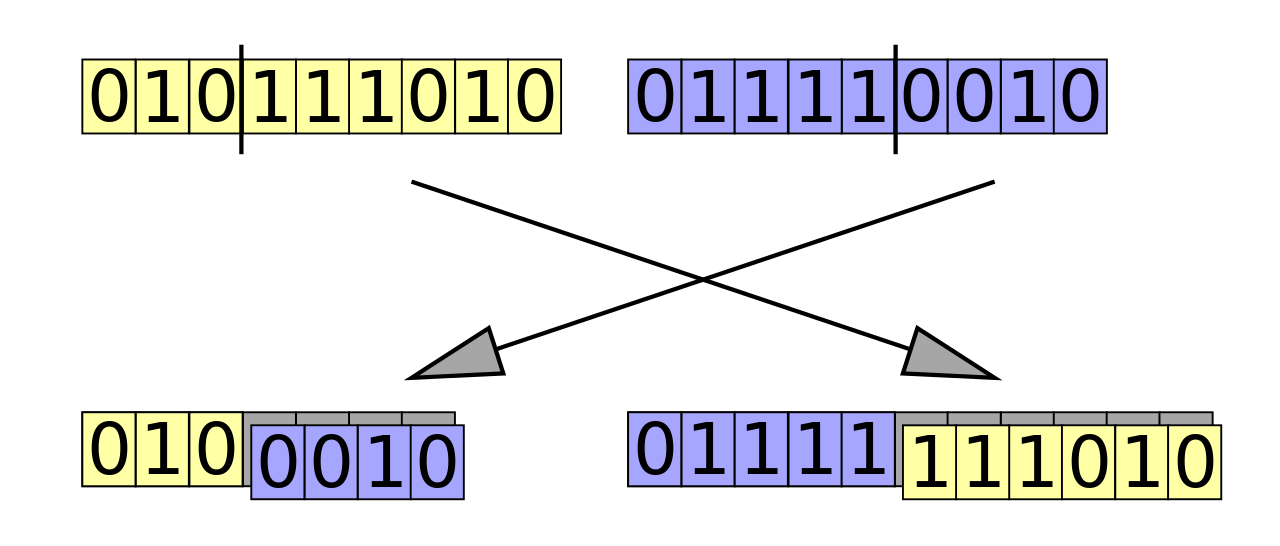
\includegraphics[width=9cm,height=5cm,keepaspectratio]{crossover.png}}
	\caption{Operador de cruce SPX}
	\label{fig:crossover}
\end{figure}

\subsection{Operadores de mutación}
Los operadores de mutación consisten en modificar un individuo modificando uno de sus genes heredados de alguno de sus padres.
A partir de una probabilidad de mutación dada por el usuario, se determina si se realizará la mutación y se intercambiará el valor de uno de los genes
por el contrario (torneo binario).\\
Considerando la probabilidad de mutación del problema, haremos uso de la siguiente operación:

% Inverse of gene length plus gene number
\begin{equation}
	p_m = \frac{1}{g_n \cdot g_l}
\end{equation}


\subsection{Algoritmo genético \textit{Steady State} (ssGA)}
ssGA es una implementación de un algoritmo genético de estado estacionario. Con los siguientes pasos de forma iterativa:

\begin{enumerate}
	\item Se genera una población inicial de individuos.
	\item Se evalúa el \textit{fitness} de cada individuo de la población.
	\item Se seleccionan dos individuos haciendo uso de un \textbf{torneo binario} (\cite{ref_tournament}).
	\item Usando el operador de cruce \textbf{SPX} (\cite{ref_spx}), se genera un nuevo individuo.
	\item Al nuevo individuo, se le aplica el operador de mutación binaria.
	\item Evaluar el \textit{fitness} del nuevo individuo.
	\item Se reemplaza el nuevo individuo en la población por el individuo que obtuvo el menor valor de \textit{fitness}.
\end{enumerate}

\section{Estudio experimental}

Para realizar el sigueinte estudio experimental, se ha usado las instancias para el problema de la mochila
que se pueden encontrar en la siguiente \cite{ref_or_library}. Se ha definido un programa que nos permite leer
la instancia y ejecutar el algoritmo genético para todas los problemas de la instancia. Estos problemas fueron
definidos en el siguiente \cite{ref_balas} \textit{paper}. \\
Para comenzar, se ha decidido ejecutar cien iteraciones a cada uno de los siete problemas descritos en la entrada del problema,
obteniendo un total de setecientas iteraciones. Para ello se ha buscando un equilibrio del tamaño de la población
y el número de generaciones máximas. Por tanto, se ha configurado el algoritmo con los siguientes parámetros de ejecución:
\begin{itemize}
	\item \textbf{Tamaño de la población}: 512
	\item \textbf{Número máximo de generaciones}: 50000
	\item \textbf{Número de repeticiones} 30
	\item \textbf{Porcentaje de cruce}: rango de cuatro números comprendido en $\numrange[range-phrase = --]{0.5}{0.9}$.
	\item \textbf{Modificador del porcentaje de mutación}:  producto cuyo valor está en el rango de cuatro números comprendidod en $\numrange[range-phrase = --]{0.8}{1.0}$.
\end{itemize}

\noindent
Una vez ejecutado el programa sobre los siete problemas, se ha obtenido una tabla con los resultados obtenidos (Tabla ~\ref{tab:results}).
\begin{table}
	\centering
	\begin{tabular}{rrrrr}
		\hline
		\textbf{Resultados} & \textbf{Min ft} & \textbf{Media ft} & \textbf{Max ft} & \textbf{D. Típica} \\
		\hline
		\textbf{Problema 1} & 3800.00         & 3800.00           & 3800.00         & 0.0000             \\
		\hline
		\textbf{Problema 2} & 8706.10         & 8706.10           & 8706.10         & 0.0000             \\
		\hline
		\textbf{Problema 3} & 4015.00         & 4015.00           & 4015.00         & 0.0000             \\
		\hline
		\textbf{Problema 4} & 6060.00         & 6118.60           & 6120.00         & 4.9978             \\
		\hline
		\textbf{Problema 5} & 12300.00        & 12391.04          & 12400.00        & 14.8815            \\
		\hline
		\textbf{Problema 6} & 10375.00        & 10564.04          & 10618.00        & 41.0814            \\
		\hline
		\textbf{Problema 7} & 16311.00        & 16455,09          & 16537.00        & 50.1717            \\
	\end{tabular}

	\caption{Resultados de los problemas.}
	\label{tab:results}
\end{table}

Se pueden obtener las siguientes conclusiones:
\begin{enumerate}
	\item Los problemas más pequeños son resueltos perfectamente por el algoritmo con el 100\% eficacia.
	\item Comenzamos a obtener una eficacia inferior al 100\% en el problema nº 4 pero muy cercana a la solución óptima (\textit{fitness} de 6060 versus 6120).
	\item La desviación típica de los resultados es cero en problemas pequeños haciendose mayor a medida que vamos aumentando el tamaño de la población en cada iteración.
\end{enumerate}

\noindent
Teniendo en cuanta los anteriores resultados, se ha decidido profundizar más realizando un estudio en la busqueda del óptimo y un estudio de la detención de la convergencia.

\subsection{Estudio en la busqueda del óptimo}\label{sec:opt}
En dicha subsección, se va a hacer un analisis de los resultados obtenidos en busca de la solución óptima. Para ello, se va a reducir el analisis a los siguientes parámetros:
\begin{itemize}
	\item Se realizará sobre los problemas 4 y 5.
	\item Porcentaje de cruce: rango de dos elementos comprendido en $\numrange[range-phrase = --]{0.5}{0.6}$.
	\item Modificador del porcentaje de mutación: rango de dos elementos comprendidos en $\numrange[range-phrase = --]{0.8}{1.0}$.
\end{itemize}

\noindent
A partir de estos datos, se ha analizado como afecta los porcentajes de cruce y mutación en la eficacia del algoritmo. Inicialmente se estudia el primero.
A razón de las 30 muestras y de las 480 combinaciones que se han realizado, una resultados más que aceptables son:
\begin{itemize}
	\item \textbf{Porcentaje de cruce}: 0.77
	\item \textbf{Modificador de la mutación}: 0.3 ó 0.4
	\item \textbf{Eficacia}: 0.7
	\item \textbf{Iteraciones medias}: 20263
\end{itemize}

\noindent
Haciendo uso de ambos modificadores, hemos obtenido una eficacia en la obtención de la solución óptima del 70\%. El algoritmo tiene un buen rendimiento con este problema,
dando soluciones óptimas y rápidas en pocas iteraciones (\~7518) pero viendose lucrado por la eficacia.

\noindent
Una posible alternativa, con mucho mayor eficacia, sería tomar una combinación de parámetros que nos ha arrojado un 100\% de eficacia en el problema 4.
\begin{itemize}
	\item \textbf{Porcentaje de cruce}: 0.63
	\item \textbf{Porcentaje de mutación}: 0.03
	\item \textbf{Eficacia}: 1.0
	\item \textbf{Iteraciones médias}: 7563
\end{itemize}

\begin{figure}
	\centering
	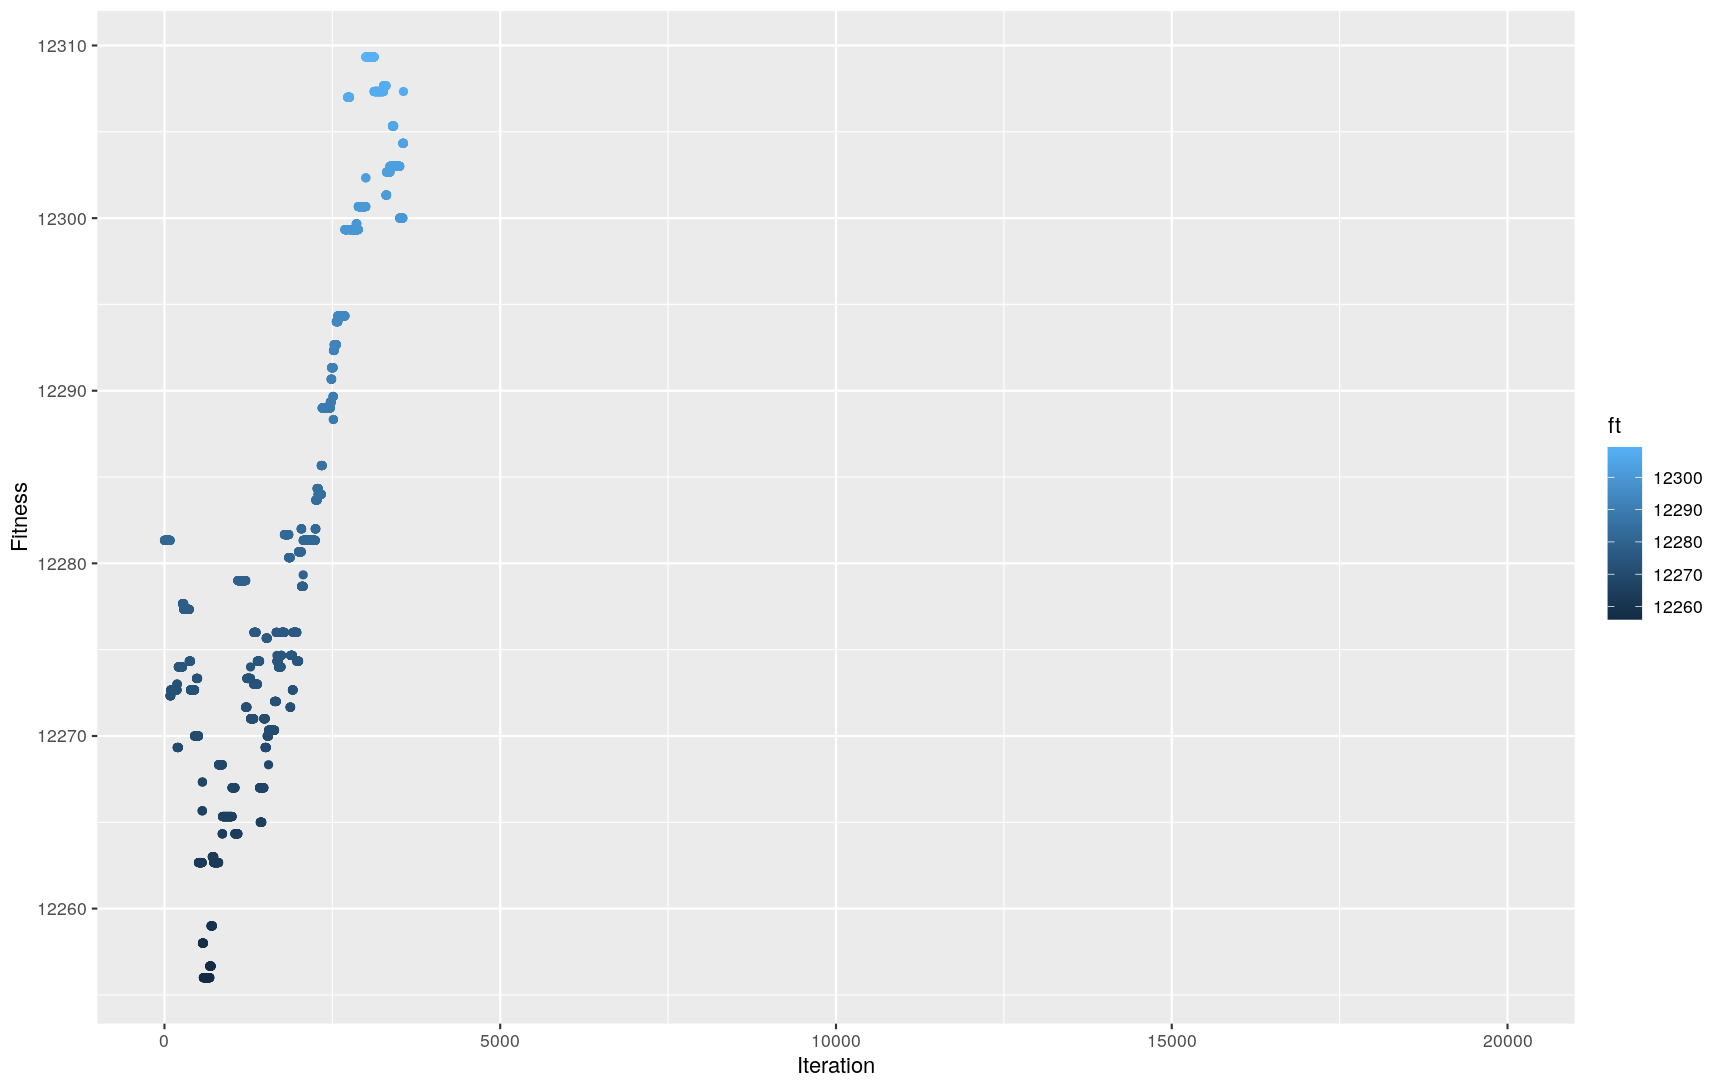
\includegraphics[width=1.0\textwidth]{graphic_optimal}
	\caption{Progreso con un porcentaje de cruce 0.63 y un porcentaje de mutación de 0.03.}
	\label{fig:results_opt_crossover_0.77_mut_0.3}
\end{figure}

\noindent
Tal como se puede observar, los resultados son perfectos, encontrando siempre la solución óptima pero tendiendo a necesitar
alguna iteración más para alcanzarla, con respecto a la anterior solución. Si analizamos de forma gráfica el resultado obtenido(Figura \ref{fig:results_opt_crossover_0.77_mut_0.3}),
se puede observar que el algoritmo ha convergido a la solución óptima en la iteración nº 7563 como máximo.\\
Inicialmente, se obtiene un resultado relativamente bueno, las próximas iteraciones se ve inmerso en una busqueda local hasta que en la iteración \~500 empieza a mejorar de forma notable.\\
En resumen, la primera solución nos aporta la ventaja de que el algoritmo tiene un buen rendimiento manteniendo un buen rango de eficacia
a costa de necesitar menor iteraciones para alcanzar un solución cercana a la óptima. Por otro lado,
la alternativa que se ha tomado es la que nos ha arrojado una eficacia
más alta, con un número de iteraciones más alto de media, pero una menor dispersión en el número de iteraciones necesarias para alcanzar la solución óptima.


\subsection{Estudio en la detención de la convergencia}
En este apartado se va a tratar de analizar el comportamiento del algoritmo en el caso de que el problema sea un problema lo suficientemente
grande que dificulte la convergencia en la solución óptima. Para ello, se va a reducir el analisis a los siguientes parámetros:

\begin{itemize}
	\item Se trabajará sobre el problema más complejo, el nº 6.
	\item Porcentaje de cruce: rango de dos elementos comprendido en $\numrange[range-phrase = --]{0.5}{0.6}$.
	\item Modificador del porcentaje de mutación: rango de dos elementos comprendidos en $\numrange[range-phrase = --]{0.8}{1.0}$.
\end{itemize}

Partiendo de los datos obtenidos en la ejecución máxima descrita con anteriorad en \ref{sec:opt}, se ha observado que el algoritmo tiende a converger
si alguno de los parámetros de cruce y mutación busca una solución local que coincide con la óptima. Visualizamos este comportamiento en la Figura \ref{fig:results_crossover_0.5_mut_0.016}.
En el gráfico observamos la media de la \textit{fitness} en las diferentes iteraciones. En las primeras iteraciones, hay un par de pruebas que 
se aproximan muy rápido a la solución óptima. A medida de que alcanzan la solución, vamos comprobando que la dispersión se mantiene estable en varios rangos, por ejemplo,
[15500, 16000]. Como se puede comprobar, el algoritmo intenta mejorar en cada iteración realizando saltos escalonados en el valor final de la \textit{fitness}.
A medida que las iteraciones van avanzando, la dispersión aumenta en las zonas de soluciones locales, y se ve reducido en las zonas de soluciones óptimas y peores soluciones.

De tal analisis podemos deducir que un algoritmo evolutivo tiende a converger en una solución óptima o muy cercana a ella.

% haciendo los siguientes parámetros:
% \begin{itemize}
% 	\item \textbf{Porcentaje de cruce}: 0.50 // 0.90
% 	\item \textbf{Porcentaje de mutación}: 0.02
% \end{itemize}
% Se han descartado los anteriores valores debido a que, tanto si el porcentaje de cruce es mínimo como máximo, el algoritmo tiende a converger, siendo irrelevante para el problema que se está tratando.

\begin{figure}
	\centering
	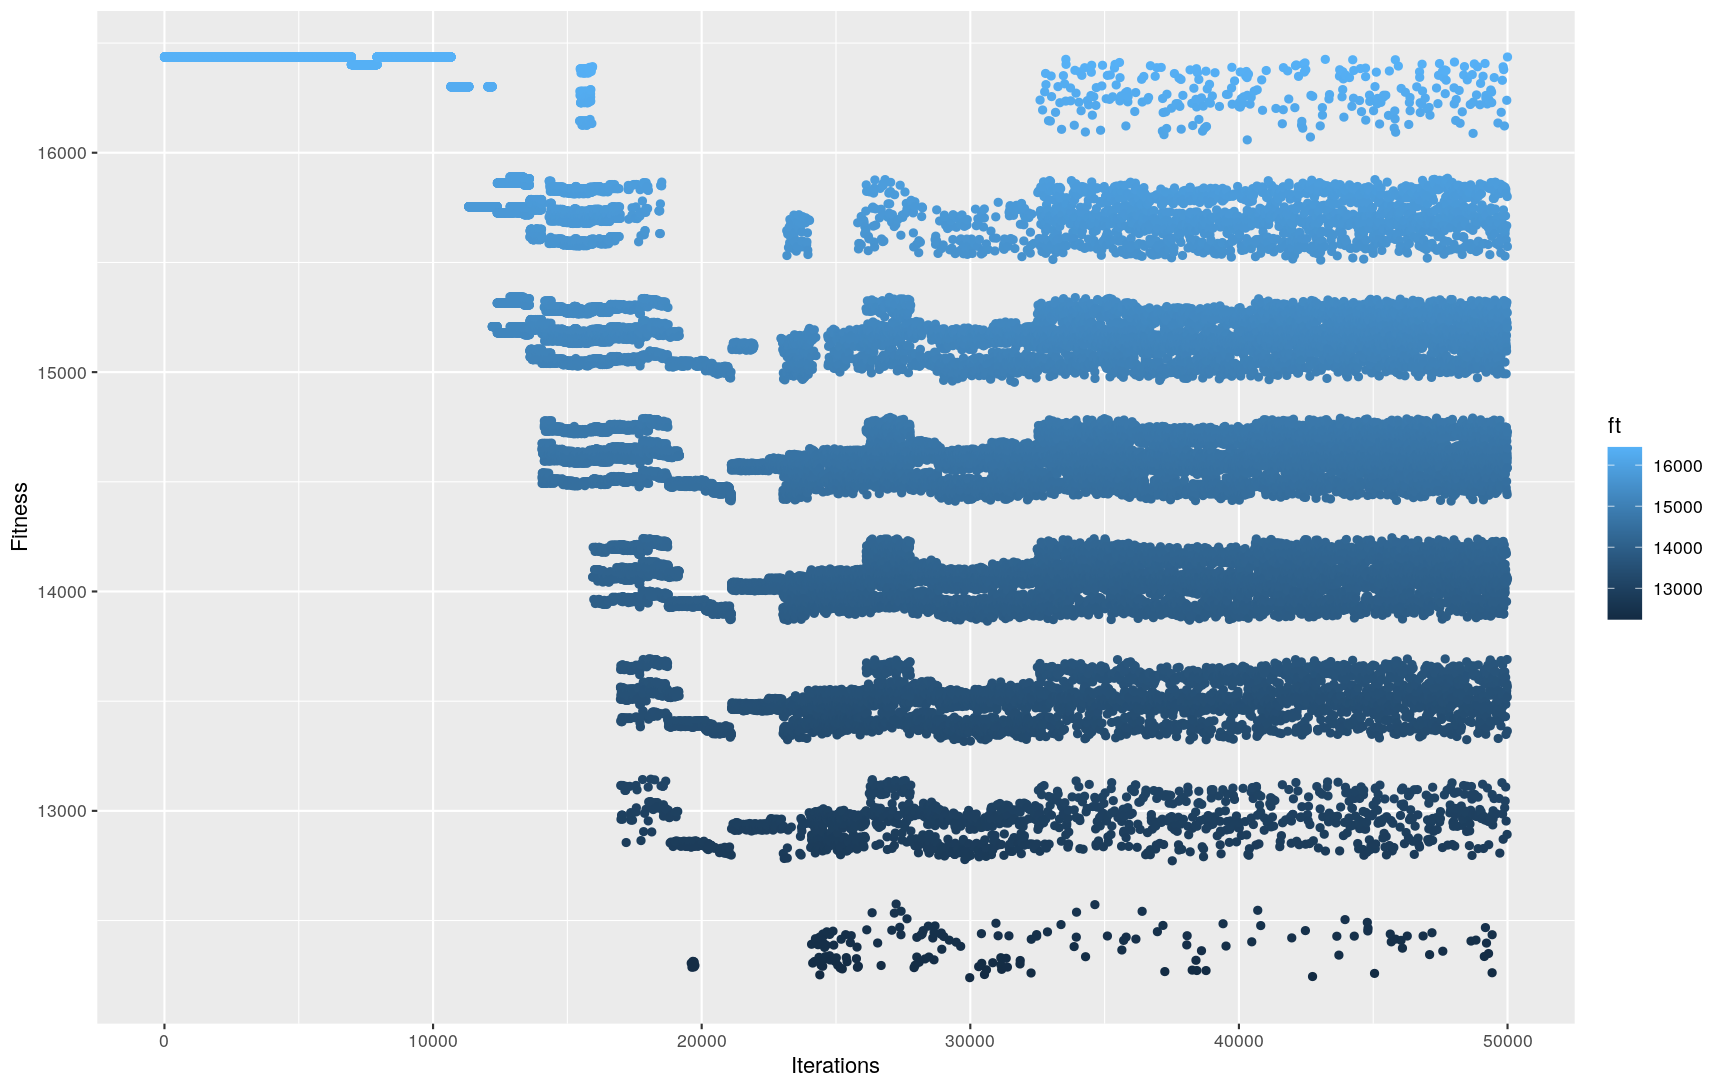
\includegraphics[width=1.0\textwidth]{graphic_dispersion}
	\caption{Progreso con un porcentaje de cruce 0.5 y un porcentaje de mutación de 0.016.}
	\label{fig:results_crossover_0.5_mut_0.016}
\end{figure}

% TODO

\section{Conclusiones}

En conclusión, haciendo balance de los datos y pruebas realizadas en los apartados anteriores, se puede decir que, los algoritmos genéticos son una herramienta muy útil para la resolución de problemas,
como el problema de mochila 0-1. Después de analizar y poder comparar los resultados de multiples pruebas, vemos unos resultados realmente buenos. Todas las soluciones obtenidas son óptimas o muy cercanas a la óptima.\\
Evidentemente, se podría intentar mejor y/o acercarse más a la solución óptima cuando no hemos obtenido los mejores resultados, pero hay que encontrar un punto equilibrio entre rendimiento y eficacia.
dado que con problemas grandes, el tiempo de computo se dispara para prácticamente no identificar soluciones mejores a las encontradas.
Por otro lado, sería importante recalcar la importancia que tiene los parámetros que nos permiten configurar el algoritmo. Una mala selección de ellos, nos puede llevar a una solución que no sea óptima.
Dado el analisis experimental hecho, podemos determinar que porcentaje de cruce y de mutación bajos nos han arrojado mejores resultados, siendo en muchos casos la solución óptima.\\
Para terminar, se podría decir que los algoritmos genéticos nos permiten resolver problemas complejos de forma muy eficiente, de forma aproximada, teniendo un mucho mejor desempeño que un algoritmo exacto.


% ---- Bibliography ----
%
% BibTeX users should specify bibliography style 'splncs04'.
% References will then be sorted and formatted in the correct style.
%
\bibliographystyle{splncs04}
\bibliography{mybibliography}
%
\begin{thebibliography}{8}
	\bibitem{ref_ssga}
	Author, E., Author: Steady State Genetic Algorithm (ssGA),
	(1999). \url{https://neo.lcc.uma.es/software/ssga/index.php}

	\bibitem{ref_spx}
	Author, T., Author, S., Author, M.: Theoretical Analysis of Simplex Crossover for Real-Coded Genetic Algorithms,
	France (2000). \url{http://www.springer.com/engineering/computational-systems-control/theoretical-analysis-of-simplex-crossover-for-real-coded-genetic-algorithms}

	\bibitem{ref_tournament}
	Tournament selection,
	(2021). \url{https://en.wikipedia.org/wiki/Tournament_selection}

	\bibitem{ref_balas}
	Author, C. C. :Computational experience with variants of the Balas algorithm applied to the selection of R\&D projects,
	(1967). \url{https://en.wikipedia.org/wiki/Tournament_selection}

	\bibitem{ref_or_library}
	Author, J., Author: OR Library,
	\url{http://people.brunel.ac.uk/~mastjjb/jeb/orlib/mknapinfo.html}


\end{thebibliography}

\end{document}
